\begin{figure}[t]
\centering
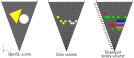
\includegraphics[width=\columnwidth]{images/volumetric/binary_decomposition}
\caption[Volumetric NED: color volume to binary volume decomposition]{Diagram shows the stages of our rendering pipeline: voxelization (see Section~\ref{sec:volumetric:Voxelization}) and binary decomposition (see Section~\ref{sec:volumetric:Decomposition}). For ease of representation, the figure depicts the rendering pipeline for a simple 2-D graphics and 6 bits-per-pixel imagery. Actual implementation uses 3-D graphics and 24 bits-per-pixel imagery. The numbers along the displayed binary volume's frustum indicate the intensity level and color of the RGB LED that illuminates the current binary image.}
%The focal planes are depicted here as equidistant from each other only for ease of representation.}
%Even though the diagram indicates the color volume and binary volume to be in a perspectively shaped volume, the computation is carried out in an orthographic (rectangular) volume. When the display presents the images, it performs an automatic inverse-perspective transformation that corrects for our computations which carried out in the rectangularly shaped volume \kishore{Shorten caption}.}
\label{fig:volumetric:binary_decomposition}
\end{figure}

